\subsection{Decision Tree Learning (DTL)}

\subsubsection{Implementasi}
Model C4.5 menerima fitur numerik dan kategorikal serta menangani nilai kosong. Pohon dibangun dari akar. Di setiap simpul, model memilih fitur untuk membagi data, lalu mengulangi prosesnya pada tiap cabang.

\paragraph{Penyiapan fitur.}
Fungsi \texttt{prepare\_dtl\_features} menandai nilai numerik negatif, jumlah tamu dewasa nol, durasi menginap nol, dan tanggal yang tidak valid sebagai nilai kosong pada kolom terkait. Nilai kosong dibiarkan agar bobotnya bisa dibagi saat pohon dibentuk. Kode angka untuk kanal pemesanan dan kategori lain tetap diperlakukan sebagai kategori.
Tanggal kedatangan dan pemesanan diubah menjadi jumlah hari sejak 1 Januari 2023 agar bisa dibandingkan. Kami menambahkan total malam, perkiraan biaya menginap, indikator nilai kosong, dan indikator seperti pemesanan tanpa permintaan khusus. Data latih dan data uji diproses secara terpisah.

\paragraph{Pemilihan pemisahan.}
Metode \texttt{fit} pada \texttt{C45DecisionTree} memberi bobot awal 1 pada setiap baris dan memanggil \texttt{\_build\_tree}. Fungsi \texttt{\_find\_split} mencoba ambang dari nilai unik fitur numerik. Setiap ambang $t$ membagi data menjadi $x\leq t$ dan $x>t$. Pada fitur kategorikal, setiap kategori yang muncul mendapat satu cabang.

Gain dihitung dari penurunan entropi pada baris yang nilainya diketahui, lalu dikalikan dengan proporsi bobot baris tersebut. Gain ratio membagi gain dengan \textit{split information}, yaitu entropi dari pembagian bobot ke tiap cabang serta kelompok nilai kosong. Dari kandidat terbaik tiap fitur, model memilih gain ratio tertinggi di antara kandidat dengan gain setidaknya sebesar rata-rata.

\paragraph{Nilai kosong dan prediksi.}
Di \texttt{\_build\_tree}, baris yang nilainya kosong dimasukkan ke semua cabang. Bagian bobot yang diterima setiap cabang mengikuti proporsi bobot dari baris yang nilainya diketahui.

\noindent\begin{minipage}{\linewidth}
\begin{lstlisting}
for branch, rows in groups.items():
    fraction = weights[rows].sum() / known_weight
    selected = rows | missing
    child_weights = weights[selected]
    child_weights[missing[selected]] *= fraction
    child = _build_tree(
        X[selected],
        y[selected],
        child_weights,
        features,
        n_classes,
        next_depth,
        min_branch_weight,
    )
    node["children"][branch] = (child, fraction)
\end{lstlisting}
\end{minipage}

\texttt{predict\_proba} mengikuti cabang yang sesuai hingga mencapai daun. Saat nilainya kosong atau kategorinya belum muncul pada simpul itu, probabilitas dari tiap cabang dirata-ratakan sesuai bobot. Pada v4, kedalaman maksimum adalah 16. Sebuah pemisahan hanya dipakai jika minimal dua cabang masing-masing punya bobot data yang diketahui sebesar 7 atau lebih. \texttt{predict} memberi label batal jika probabilitas kelas 1 mencapai $0{,}48$.

\subsubsection{Hasil dan Perbandingan dengan scikit-learn}
Ketiga model diuji pada 5.475 baris validasi yang sama. Data dibagi secara terstratifikasi (80\% latih dan 20\% validasi) dengan \texttt{random\_state=824}. Metrik utama yang dipakai adalah Macro F1, yaitu rata-rata F1 kelas batal dan tidak batal.

Pembanding \texttt{DecisionTreeClassifier} memakai kriteria \texttt{entropy} dan kedalaman maksimum 16. Dari tiga nilai \texttt{ccp\_alpha} yang dicoba, $0{,}0005$ memberi Macro F1 validasi tertinggi. Median, modus, dan pengodean \textit{one-hot} ditentukan dari data latih, lalu dipakai pada data validasi.

\begin{table}[!htbp]
  \centering
  \caption{Hasil validasi DTL pada pemisahan 80:20.}
  \label{tab:dtl-validation}
  \begin{tabular}{@{}lrr@{}}
    \toprule
    Model & Akurasi & Macro F1 \\
    \midrule
    C4.5 v3 & 0,85753 & 0,83744 \\
    C4.5 v4 & 0,85717 & \textbf{0,83842} \\
    scikit-learn & 0,85425 & 0,83183 \\
    \bottomrule
  \end{tabular}
\end{table}

Macro F1 v4 naik sekitar 0,10 poin persentase dari v3. Akurasi keduanya hampir sama (Tabel~\ref{tab:dtl-validation}). Pada Gambar~\ref{fig:dtl-confusion}, v4 mengenali 1.414 pembatalan dan scikit-learn mengenali 1.339. Jumlah pemesanan yang keliru diprediksi batal adalah 402 pada v4 dan 343 pada scikit-learn.

\begin{figure}[!htbp]
  \centering
  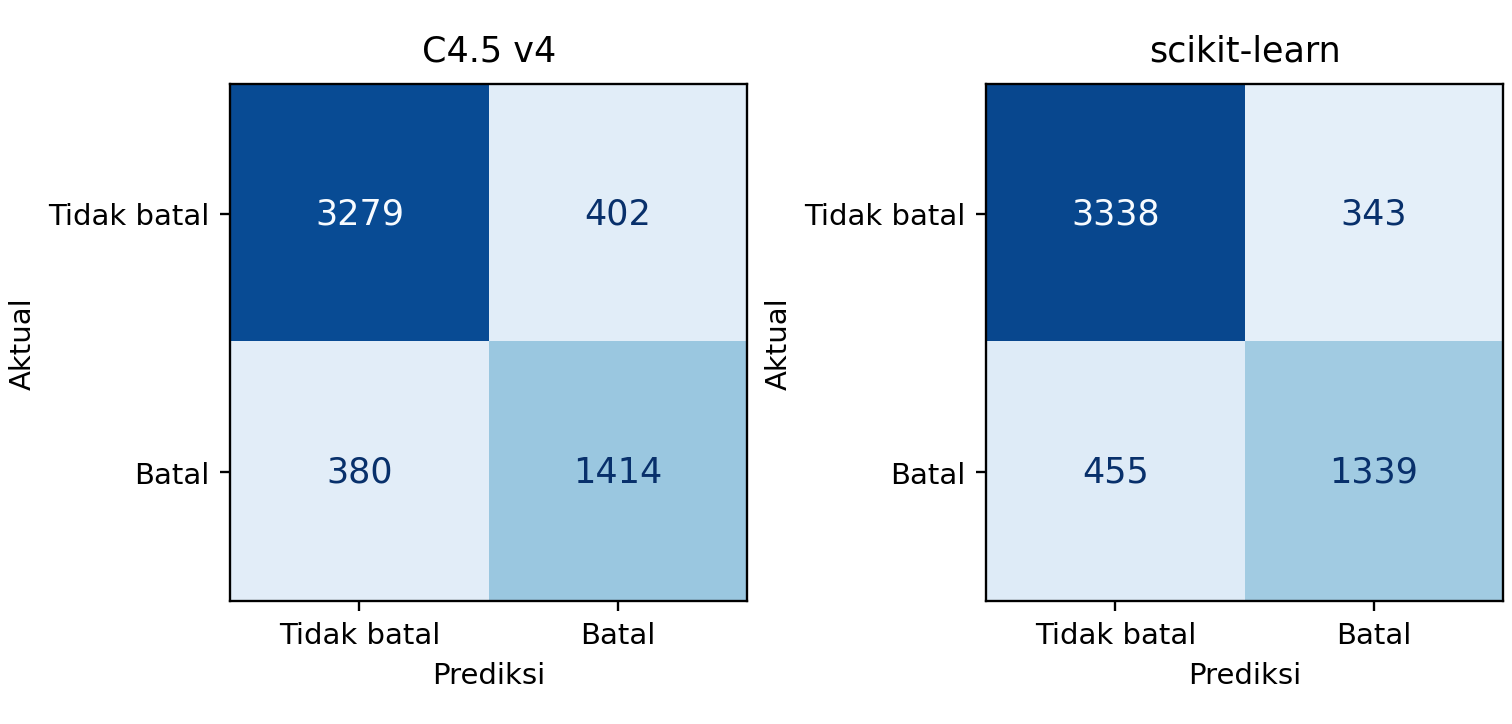
\includegraphics[width=0.94\linewidth]{assets/dtl/dtl_confusion.png}
  \caption{Matriks kebingungan C4.5 v4 dan scikit-learn pada data validasi yang sama.}
  \label{fig:dtl-confusion}
\end{figure}

Untuk submisi, v4 dilatih ulang pada seluruh data latih. Prediksi sebelum dan sesudah model disimpan dan dimuat kembali identik. CSV berisi 6.844 prediksi dengan urutan ID sesuai templat submisi. Skor publik Kaggle untuk v4 adalah 0,84191 (Macro F1).

\subsubsection{Visualisasi Pohon}
Gambar~\ref{fig:dtl-tree} menampilkan pohon v4 yang dipakai untuk submisi. Fungsi \texttt{plot\_dtl\_tree} menelusuri pohon per tingkat dari akar. Pada simpul yang sama, cabang berbobot lebih besar digambar dulu. Parameter \texttt{top\_n} membatasi jumlah cabang yang terlihat. Di gambar ini batasnya 10.
Pada akar, model membagi pemesanan lewat \texttt{days\_before\_arrival}. Bobot kelas batal sekitar 24\% pada pemesanan yang dibuat paling lama 152 hari sebelum kedatangan dan 70\% pada pemesanan yang dibuat lebih awal.

\begin{figure}[!htbp]
  \centering
  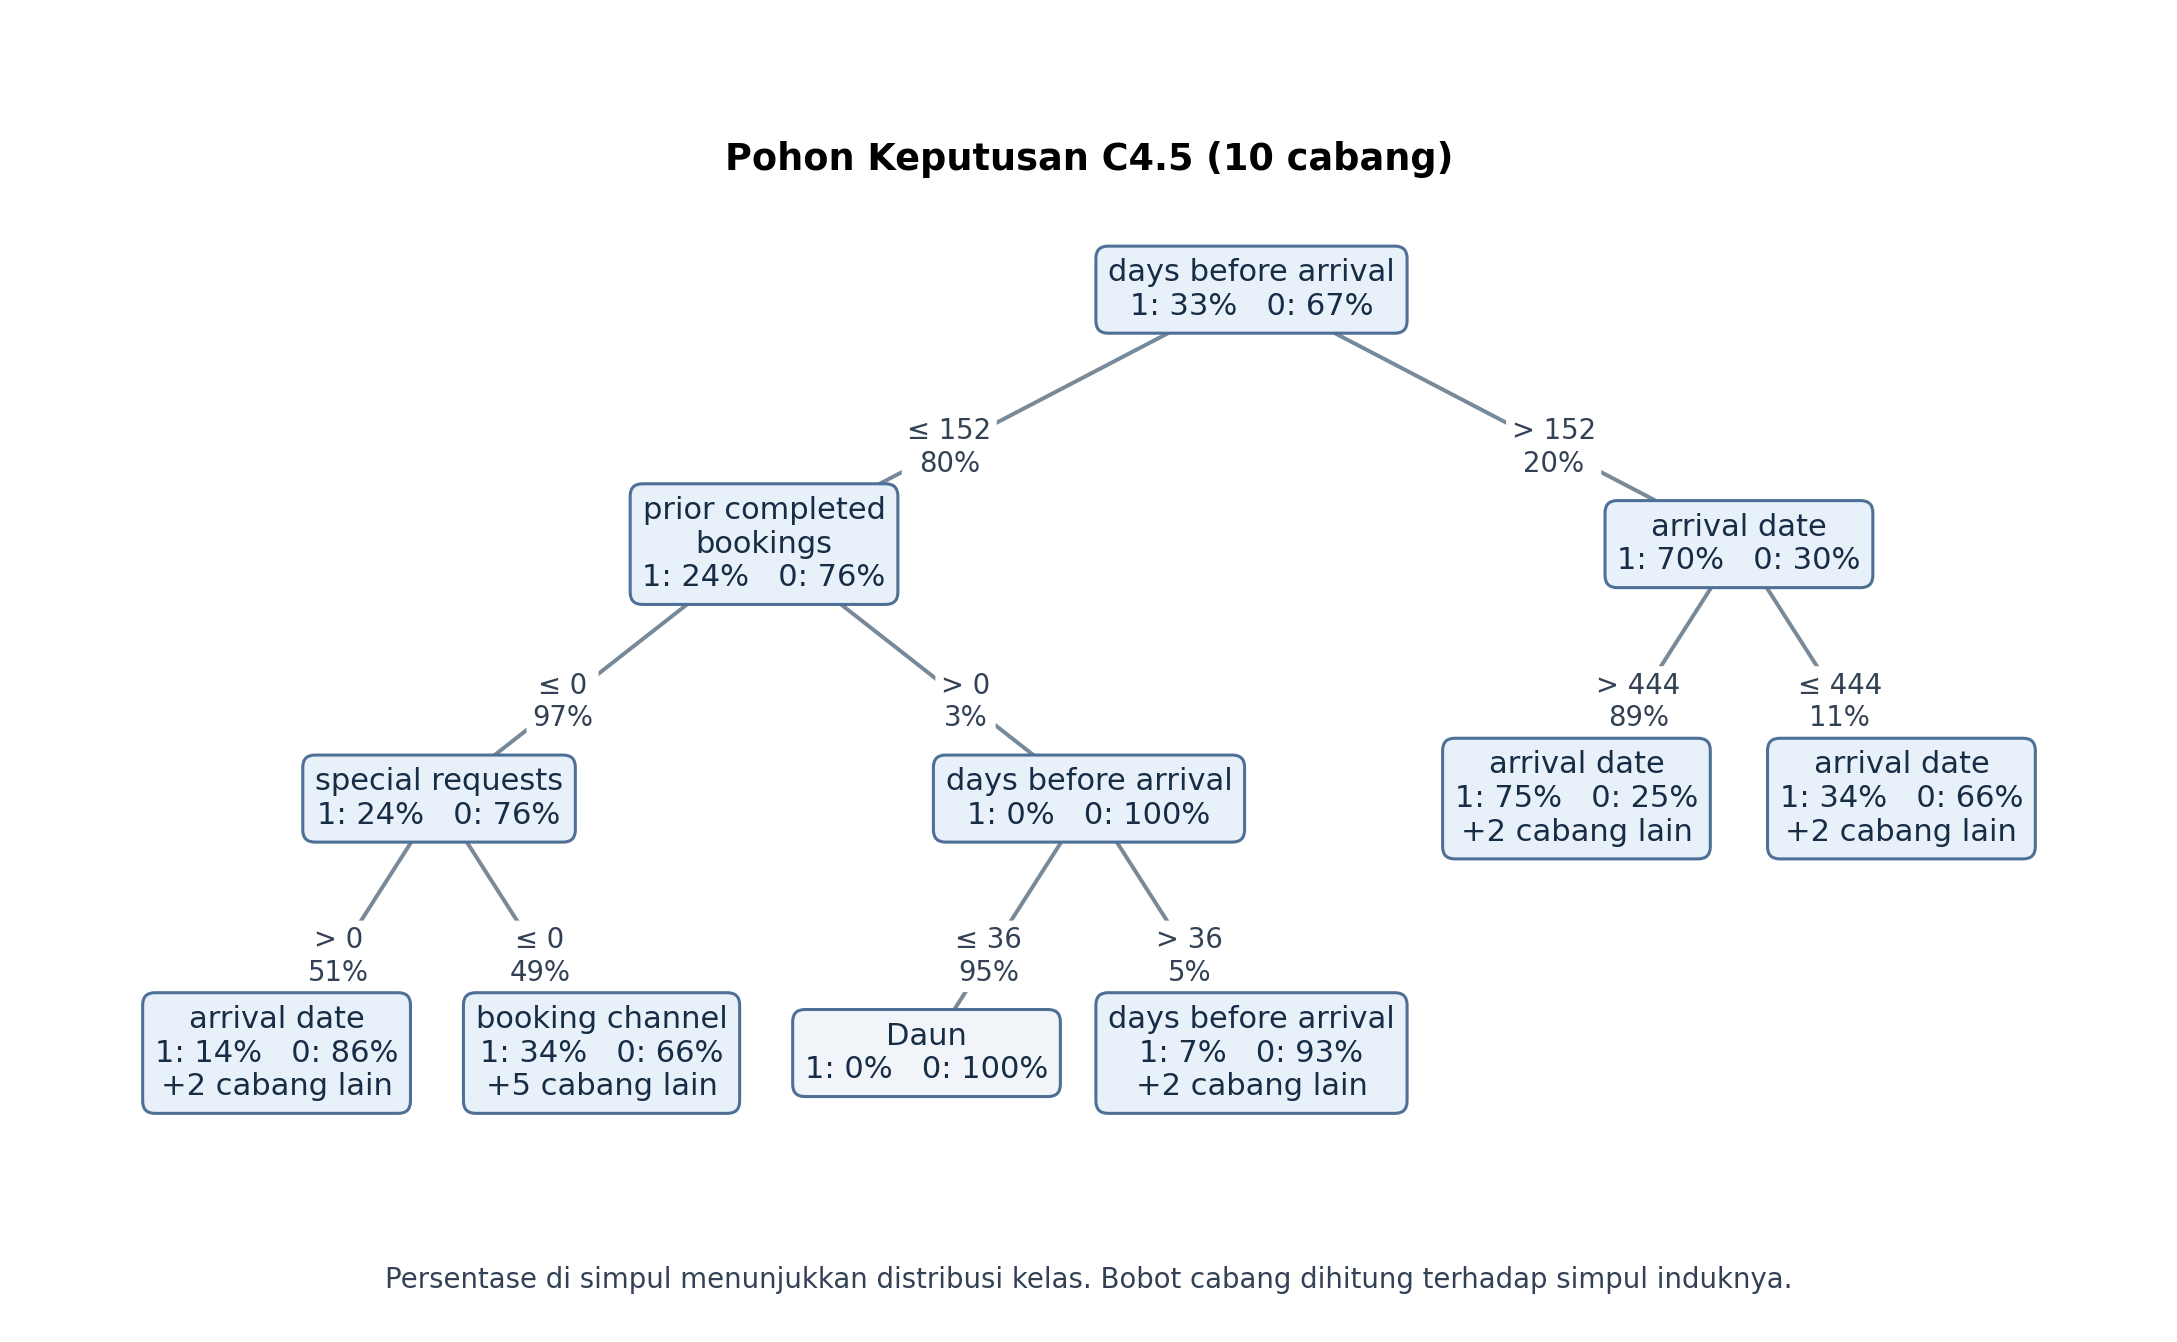
\includegraphics[width=\linewidth]{assets/dtl/dtl_tree.png}
  \caption{Sepuluh cabang awal pohon C4.5 v4. Kelas 0 berarti tidak batal dan kelas 1 berarti batal.}
  \label{fig:dtl-tree}
\end{figure}
